%TCIDATA{LaTeXparent=0,0,relatorio.tex}
\ifx\compilewholereport\undefined
	\documentclass[11pt,a4paper,oneside]{book}
	
	% Escolher um dos seguintes formatos:
	\usepackage{ft2unb} % segue padrão de fontes do Latex
	
	% Pacotes
	\usepackage{graphicx}
	\usepackage{amsfonts}
	\usepackage{amsmath}
	\usepackage{amssymb}
	\usepackage[thmmarks,amsmath]{ntheorem}
	\usepackage{boxedminipage}
	\usepackage{theorem}
	\usepackage{fancybox}
	\usepackage{fancyhdr}
	\usepackage{url}
	\usepackage{afterpage}
	\usepackage{color}
	\usepackage{colortbl}
	\usepackage{rotating}
	\usepackage{makeidx}
	\usepackage{indentfirst}
	\usepackage{bibentry}
	\usepackage{subcaption}
	\usepackage{todonotes}
	\presetkeys{todonotes}{inline}{}
	
	\begin{document}
	\frontmatter
	\tableofcontents
	\mainmatter
	
	%%%%%%%%%%%%%%%%%%%%%%%%%%%%
	%%%%%%%% Apagar coisas acima
	%%%%%%%%%%%%%%%%%%%%%%%%%%%%
\fi
                      
\chapter{Revis\~{a}o Bibliogr\'{a}fica}\label{CapRevisaoBibliografica}

% Resumo opcional. Comentar se não usar.
\resumodocapitulo{Este capítulo visa apresentar o estado-da-arte da reconfiguração dinâmica e da auto-reconfiguração e as ferramentas necessárias para sua realização.}

%\section{Introdução}
\vspace{0.8cm}
Os temas reconfiguração dinâmica, parcial e autoreconfiguração 

\section{Classes de Reconfigura\c{c}\~ao}
Com a chegada de CPLDs e FPGAs, requisitos cada vez mais complexos foram sendo introduzidos ao projeto de sistemas digitais.
Tais requisitos for\c{c}aram as ferramentas de s\'i­ntese a suportar diferentes classes de reconfigura\c{c}\~ao.
Note que reconfigura\c{c}\~ao diz respeito, como dito anteriormente, a modifica\c{c}\~ao do comportamento, ou configura\c{c}\~ao, de um dispositivo reconfigur\'avel.

\subsection{Reconfigura\c{c}\~ao Total}
A reconfigura\c{c}\~ao total, herdada da tecnologia tradicional, compreende a mudan\c{c}a do comportamento de todo o dispositivo reconfigur\'avel, sem exce\c{c}\~ao de blocos l\'ogicos.
Tal reconfigura\c{c}\~ao \'e bastante dispendiosa, visto que maior parte das alterações realizadas são incrementais e dizem respeito \`a apenas uma pequena parte do dispositivo.
Apesar disto, todos os FPGAs d\~ao suporte a este tipo de reconfigura\c{c}\~ao.

\subsection{Reconfigura\c{c}\~ao Parcial}
A reconfigura\c{c}\~ao parcial, ao contr\'ario da reconfigura\c{c}\~ao total, diz respeito \`a programa\c{c}\~ao de apenas parte de um dispositivo reconfigur\'avel \cite{Hauck2007}.
Para tal, faz-se necess\'ario a divis\~ao do dispositivo nas chamadas parti\c{c}\~oes, cada uma com sua configura\c{c}\~ao individual.
Desta forma, mudan\c{c}as feitas em uma parti\c{c}\~ao n\~ao afetam as outras, acelerando o processo de s\'i­ntese e programa\c{c}\~ao.
Outro processo que \'e acelerado \'e o de roteamento, uma vez que o particionamento introduz limita\c{c}\~oes no mapeamento das fun\c{c}\~oes.
Nem todos os FPGAs d\~ao suporte a este tipo de reconfigura\c{c}\~ao, que pode ser realizado tanto de forma dinâmica (\ref{sss:dinamica}) quando estática (\ref{sss:estatica}).

\subsection{Reconfigura\c{c}\~ao Est\'atica}
\label{sss:estatica}
O termo reconfigura\c{c}\~ao est\'atica se refere a programa\c{c}\~ao de um dispositivo reconfigur\'avel enquanto ele n\~ao estiver executando.
No caso em que alguma programa\c{c}\~ao j\'a tenha sido transferida para ele e ele a esteja executando, esta \'e parada para que o dispositivo seja configurado novamente.
Por ser mais f\'acil de ser implementada e n\~ao necessita de circuitos adicionais, todos os FPGAs d\~ao suporte a este tipo de reconfigura\c{c}\~ao.

\subsection{Reconfigura\c{c}\~ao Din\^amica}
\label{sss:dinamica}
A reconfigura\c{c}\~ao din\^amica acontece frente \`a necessidade de reprograma\c{c}\~ao parcial do dispositivo sem que ele pare de funcionar.
As funcionalidades modificadas s\~ao interrompidas e substituidas sem afetar o funcionamento do todo.
Normalmente este processo, quando n\~ao associado a autorreconfigura\c{c}\~ao, \'e realizado atrav\'es de um circuito externo à FPGA, tal como um controlador, um microcontrolador, ou mesmo um computador, como apresentado na figura \ref{fig:rexterna}.
Quase todos os FPGAs modernos d\~ao suporte a esta tecnologia.

\begin{figure}[htp]
\centering
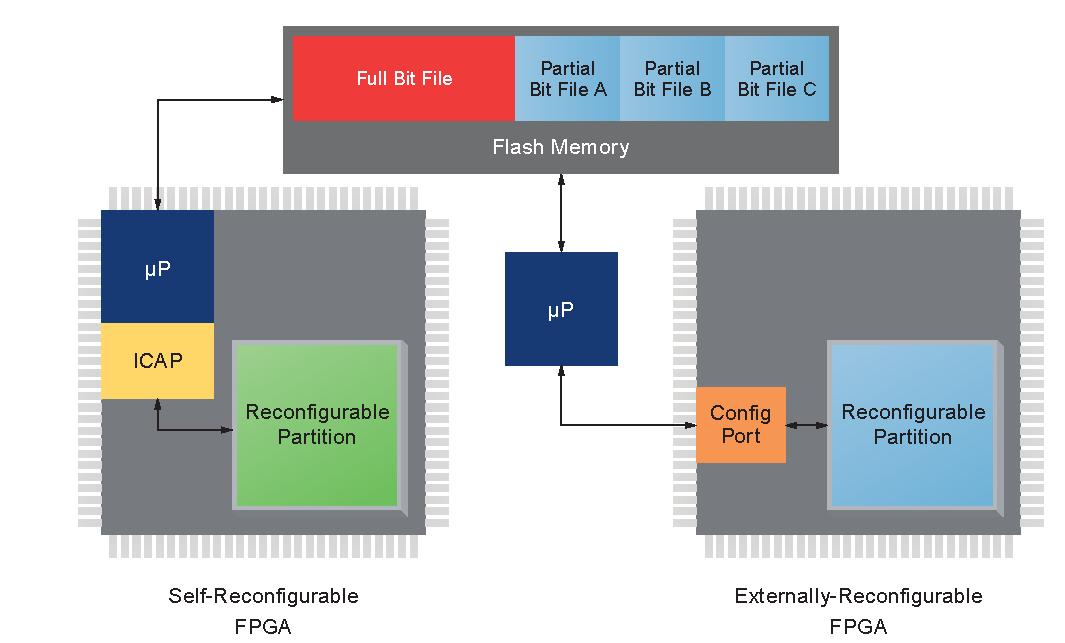
\includegraphics[width=0.8\textwidth]{fig/c1_introducao/reconf_externa.pdf}
\caption{Imagem ilustrativa para diferenciação entre autorreconfiguração e reconfiguração externa, extraido de \cite{wp374}.}
\label{fig:rexterna}
\end{figure}

É implicito o uso da reconfiguração parcial com a reconfiguração dinâmica, uma vez que faz pouco sentido reconfigurar todo o FPGA enquanto ela ainda está em execução.
Note que este tipo de reconfiguração em geral também necessita de uma parte permanentemente est\'atica, para interfacear com o circuito controlador.
Esta parti\c{c}\~ao est\'atica \'e respons\'avel pelo menos por controlar a comunica\c{c}\~ao com o circuito controlador.

Vale lembrar que a este tipo de reconfiguração, apesar de abrir muitas possibilidades, introduz uma necessidade de preocupação com \textit{overheads} de reconfiguração \cite{Hauck2007}.
Este \textit{overhead} é proporcional ao tamanho da partição que se deseja modificar e inversamente proporcional às velocidades das interfaces de reconfiguração.
Tal fator pode se tornar crucial na escolha entre o uso desta tecnologia ou alguma outra alternativa, possivelmente multiplexada.
Note que existem outros fatores que influenciam na opção por reconfiguração dinâmica, tais como preço, capacidade e potência, dentre outros, que não serão considerados aqui.

\subsection{Autorreconfigura\c{c}\~ao}
Modalidade de reconfigura\c{c}\~ao din\^amica parcial onde a reconfigura\c{c}\~ao do dispositivo \'e decidida por uma l\'ogica pertencente a ele mesmo.
Normalmente usa-se um microcontrolador ou uma m\'aquina de estados finitos para controlar a mudan\c{c}a de configura\c{c}\~oes.
Este tecnologia \'e nova e ainda representa uma forte \'area de pesquisa.
Por isso n\~ao s\~ao todos os FPGAs que d\~ao suporte a este tipo de reconfigura\c{c}\~ao.

Para que a autorreconfigura\c{c}\~ao aconte\c{c}a, os \textit{bitstreams}, resultado da sintetiza\c{c}\~ao, devem ser passados para uma mem\'oria acess\'i­vel ao FPGA durante a execu\c{c}\~ao do mesmo.
O circuito controlador identifica ent\~ao um padr\~ao que defina a necessidade de reconfigura\c{c}\~ao e transfere o \textit{bitstream} correspondente a esta nova necessidade para a parti\c{c}\~ao destino, que assim muda seu comportamento.
Note que para tal, as entradas e sa\'i­das das parti\c{c}\~oes tem que ser fixas, para que a mudan\c{c}a nas configura\c{c}\~oes das parti\c{c}\~oes n\~ao danifique o FPGA em si.

\todo{Apresentar o estado-da-arte}

\section{Ferramentas}
Diversas ferramentas foram utilizadas para a realização deste trabalho.
Dentre eles pode-se citar os programas da Xilinx, interpretadores da linguagem Python, Perl e Tcl, compiladores de \LaTeX~e a ferramenta de controle de versão Git.
Abaixo segue uma pequena descrição sobre as ferramentas mais críticas destas.

\section{Xilinx ISE Design Suite}
O \textit{ISE Design Suite} é um conjunto de ferramentas da Xilinx para o desenvolvimento de projetos de \textit{hardware}.
Estes programas estão apresentados a seguir.

\subsection{Xilinx ISE Design Tools}
O \textit{ISE Design Tools}, disponível para os sistemas Windows XP (32 e 64 bits), Windows 7 (32 e 64 bits), Windows Server 2008 (64 bits), Red Hat Enterprise 5 e 6 (32 e 64 bits) e SUSE Linux Enterprise 11 (32 e 64 bits) \cite{ug631}, controla todos os aspectos do fluxo de projeto \cite{ug695}.
Através do \textit{Project Navigator}, sua principal ferramenta, é possivel acessar todas as configurações e ferramentas de implementação de configurações.

\paragraph{\textit{Project Navigator}} O \textit{Project Navigator} é a principal ferramenta do \textit{ISE Design Tools}.
Através dela é possível criar projetos, incluir arquivos de descrição de \textit{hardware}, seja em VHDL, Verilog ou esquemáticos, construir componentes de propriedade intelectual, impor restrições e compilá-los, dentre outras coisas.

\paragraph{iMPACT}
\paragraph{\textit{Core Generator}}

\subsection{\textit{Embedded Development Kit}}
\paragraph{Xilinx Platform Studio}
\paragraph{Xilinx Software Development Kit}

\subsection{PlanAhead}
%\subsection{ChipScope}
%\subsection{System Generator}
\subsection{Ferramentas de Linha de Comando}
\paragraph{Xilinx Sinthesis Tool (XST)}


\section{Componentes}
\section{\textit{Intellectual Property}}
\todo{Clock}
\todo{Memória DDR3, MIG, MIS}
\section{Interfaces}
\todo{SelectMAP}
\todo{ICAP e ICAPE2}

\ifx\compilewholereport\undefined
	\bibliographystyle{authordate1} 
	%\bibliography{bibliografia}
	\newsavebox\mytempbib\savebox\mytempbib{\parbox{\textwidth}{\bibliography{bibliografia}}}
	\listoftodos
	\end{document}
\fi